%%%%%%%%%%%%%%%%%%%%%%%%%%%%%%%%%%%%%%%%%%%%%%%%%%%%%%%%%%%%%%%%%%%%%%%%%%%%%%%%
%% Plantilla de memoria en LaTeX para la ETSIT - Universidad Rey Juan Carlos
%%
%% Por Gregorio Robles <grex arroba gsyc.urjc.es>
%%     Grupo de Sistemas y Comunicaciones
%%     Escuela Técnica Superior de Ingenieros de Telecomunicación
%%     Universidad Rey Juan Carlos
%% (muchas ideas tomadas de Internet, colegas del GSyC, antiguos alumnos...
%%  etc. Muchas gracias a todos)
%%
%% La última versión de esta plantilla está siempre disponible en:
%%     https://github.com/gregoriorobles/plantilla-memoria
%%
%% Para obtener PDF, ejecuta en la shell:
%%   make
%% (las imágenes deben ir en PNG o JPG)

%%%%%%%%%%%%%%%%%%%%%%%%%%%%%%%%%%%%%%%%%%%%%%%%%%%%%%%%%%%%%%%%%%%%%%%%%%%%%%%%

\documentclass[a4paper, 12pt]{book}
%\usepackage[T1]{fontenc}

\usepackage[a4paper, left=2.5cm, right=2.5cm, top=3cm, bottom=3cm]{geometry}
\usepackage{times}
\usepackage{subcaption}
\usepackage[utf8]{inputenc}
\usepackage[spanish]{babel} % Comenta esta línea si tu memoria es en inglés
\usepackage{url}
%\usepackage[dvipdfm]{graphicx}
\usepackage{graphicx}
\usepackage{float}  %% H para posicionar figuras
\usepackage[nottoc, notlot, notlof, notindex]{tocbibind} %% Opciones de índice
\usepackage{latexsym}  %% Logo LaTeX

\title{Memoria del Proyecto}
\author{Nombre del autor}

\renewcommand{\baselinestretch}{1.5}  %% Interlineado

\begin{document}

\renewcommand{\refname}{Bibliografía}  %% Renombrando
\renewcommand{\appendixname}{Apéndice}

%%%%%%%%%%%%%%%%%%%%%%%%%%%%%%%%%%%%%%%%%%%%%%%%%%%%%%%%%%%%%%%%%%%%%%%%%%%%%%%%
% PORTADA

\begin{titlepage}
\begin{center}
\begin{tabular}[c]{c c}
%
\includegraphics[bb=0 0 194 352, scale=0.25]{logo} &

\includegraphics[scale=0.25]{img/logo_vect.png} &
\begin{tabular}[b]{l}
\Huge
\textsf{UNIVERSIDAD} \\
\Huge
\textsf{REY JUAN CARLOS} \\
\end{tabular}
\\
\end{tabular}

\vspace{3cm}

\Large
MASTER UNIVERSITARIO EN VISIÓN ARTIFICIAL

\vspace{0.4cm}

\large
Curso Académico 2019/2020

\vspace{0.8cm}

Trabajo Fin de Máster

\vspace{2.5cm}

\LARGE
REALIDAD AUMENTADA CON SD-SLAM MOBILE

\vspace{4cm}

\large
Autor : Francisco Javier Palacios Fernández \\
Tutor : Eduardo Perdices Garcia y José María Cañas Plaza
\end{center}
\end{titlepage}

\newpage
\mbox{}
\thispagestyle{empty} % para que no se numere esta pagina


%%%%%%%%%%%%%%%%%%%%%%%%%%%%%%%%%%%%%%%%%%%%%%%%%%%%%%%%%%%%%%%%%%%%%%%%%%%%%%%%
%%%% Para firmar
\clearpage
\pagenumbering{gobble}
\chapter*{}

\vspace{-4cm}
\begin{center}
\LARGE
\textbf{Trabajo Fin de Grado/Máster}

\vspace{1cm}
\large
Título del Trabajo con Letras Capitales para Sustantivos y Adjetivos

\vspace{1cm}
\large
\textbf{Autor :} Nombre del Alumno/a \\
\textbf{Tutor :} Dr. Gregorio Robles Martínez

\end{center}

\vspace{1cm}
La defensa del presente Proyecto Fin de Carrera se realizó el día \qquad$\;\,$ de \qquad\qquad\qquad\qquad \newline de 20XX, siendo calificada por el siguiente tribunal:


\vspace{0.5cm}
\textbf{Presidente:}

\vspace{1.2cm}
\textbf{Secretario:}

\vspace{1.2cm}
\textbf{Vocal:}


\vspace{1.2cm}
y habiendo obtenido la siguiente calificación:

\vspace{1cm}
\textbf{Calificación:}


\vspace{1cm}
\begin{flushright}
Fuenlabrada, a \qquad$\;\,$ de \qquad\qquad\qquad\qquad de 20XX
\end{flushright}


\chapter*{}
\pagenumbering{Roman} % para comenzar la numeracion de paginas en numeros romanos
\begin{flushright}
\textit{Dedicado a \\
mi familia / mi abuelo / mi abuela}
\end{flushright}


\chapter*{Agradecimientos}
%\addcontentsline{toc}{chapter}{Agradecimientos} % si queremos que aparezca en el índice
\markboth{AGRADECIMIENTOS}{AGRADECIMIENTOS} % encabezado 


%%%%%%%%%%%%%%%%%%%%%%%%%%%%%%%%%%%%%%%%%%%%%%%%%%%%%%%%%%%%%%%%%%%%%%%%%%%%%%%%
%%%% Resumen

\chapter*{Resumen}
%\addcontentsline{toc}{chapter}{Resumen} % si queremos que aparezca en el índice
\markboth{RESUMEN}{RESUMEN} % encabezado
Hola hola

%%%%%%%%%%%%%%%%%%%%%%%%%%%%%%%%%%%%%%%%%%%%%%%%%%%%%%%%%%%%%%%%%%%%%%%%%%%%%%%%
%%%% Resumen en inglés

\chapter*{Summary}
%\addcontentsline{toc}{chapter}{Summary} % si queremos que aparezca en el índice
\markboth{SUMMARY}{SUMMARY} % encabezado




%%%% Índice de contenidos
\tableofcontents 
%%%% Índice de figuras
\cleardoublepage
%\addcontentsline{toc}{chapter}{Lista de figuras} % para que aparezca en el indice de contenidos
\listoffigures % indice de figuras
%%%% Índice de tablas
%\cleardoublepage
%\addcontentsline{toc}{chapter}{Lista de tablas} % para que aparezca en el indice de contenidos
%\listoftables % indice de tablas


%%%%%%%%%%%%%%%%%%%%%%%%%%%%%%%%%%%%%%%%%%%%%%%%%%%%%%%%%%%%%%%%%%%%%%%%%%%%%%%%
%%%%%%%%%%%%%%%%%%%%%%%%%%%%%%%%%%%%%%%%%%%%%%%%%%%%%%%%%%%%%%%%%%%%%%%%%%%%%%%%
% INTRODUCCIÓN %
%%%%%%%%%%%%%%%%%%%%%%%%%%%%%%%%%%%%%%%%%%%%%%%%%%%%%%%%%%%%%%%%%%%%%%%%%%%%%%%%

\cleardoublepage
\chapter{Introducción}
\label{sec:intro} % etiqueta para poder referenciar luego en el texto con ~\ref{sec:intro}
\pagenumbering{arabic} % para empezar la numeración de página con números
En este trabajo hacemos funcionar el algoritmo de SLAM, SD-SLAM, en dispositivos Android haciendo que todo el procesamiento de datos sea realizado por el dispositivo y en tiempo real. Además implementamos una base de Realidad Aumentada para comprobar su funcionamiento y dar pie a poder desarrollar aplicaciones con usos en la realidad. En este capitulo, hablaremos de en que bases se encuentra fundamentado este trabajo.

\section{Visión Artificial}
\label{sec:visionartificial}

La visión artificial es una rama de la inteligencia artificial que intenta conseguir información de alto nivel a partir de imágenes o videos, que luego pueda ser interpretada para realizar acciones dependiendo de las características de la información hallada, de forma automática y a través de ordenadores. Por ejemplo, para automatizar un proceso de acceso a unas instalaciones, se podría disponer de una cámara que captara la cara de las personas que quisieran entrar, contrastarla con las imágenes guardadas anteriormente de las personas que pueden acceder y decidir si la persona en cuestión tiene permiso para entrar o no.

Las investigaciones en visión artificial empezaron en la década de los 60, con la idea de conseguir la capacidad de los humanos usando su sistema visual. En 1966, se creía, que bastaría con conectar una cámara a un ordenador y preguntarle "¿Que es lo que ves?. En los 70 se formó una etapa temprana de muchos de los algoritmos de bajo nivel que utilizamos hoy en día, como pueden ser el reconocimiento de bordes en una imagen, flujo óptico o estimación del movimiento.

\begin{figure}[ht]
\centering
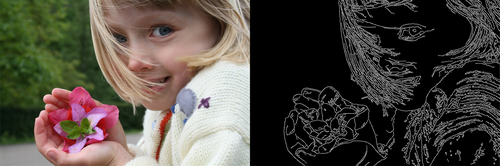
\includegraphics[scale=0.8]{img/edge_detection.png}%
\caption{Ejemplo de detector de bordes. Wikipedia-edgedetection}%
\end{figure}

Gracias a estos primeros acercamientos y al hecho de que las cámaras y ordenadores son mucho más baratos, más eficientes y más pequeños, la visión artificial a avanzado mucho en desde entonces. Hoy es fácil encontrar aplicaciones que hagan uso de una manera u otra de la visión artificial para simplificar ciertos trabajos, como puede ser OCR para digitalizar textos, detección de señales de tráfico, sistemas biométricos para reconocer la cara de una persona o realidad aumentada para medición del entorno.

\begin{figure}[ht]
\centering
\begin{subfigure}{0.3\textwidth}
  \centering
  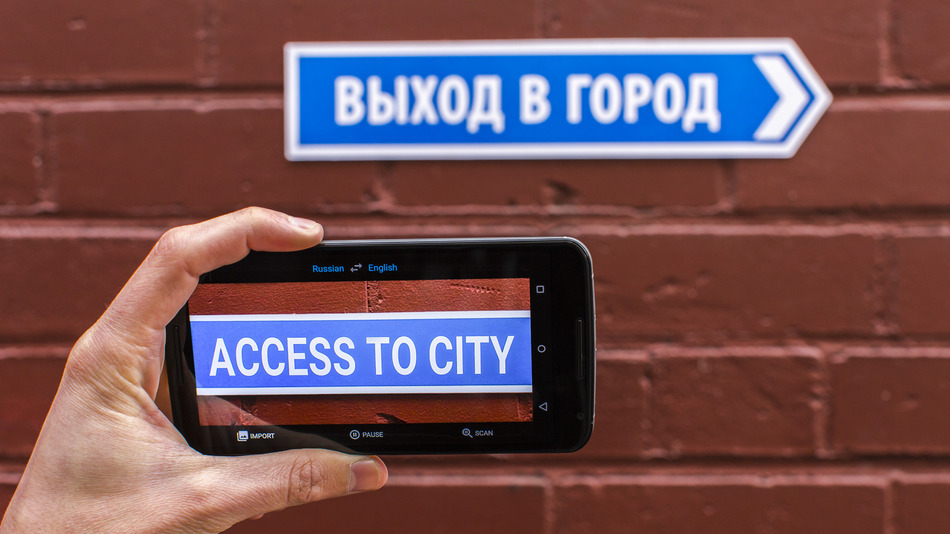
\includegraphics[scale=0.4]{img/google-translate-word-lens.jpg}
\end{subfigure}%
\qquad
\qquad
\qquad
\qquad
\qquad
\qquad
\begin{subfigure}{0.3\textwidth}
  \centering
  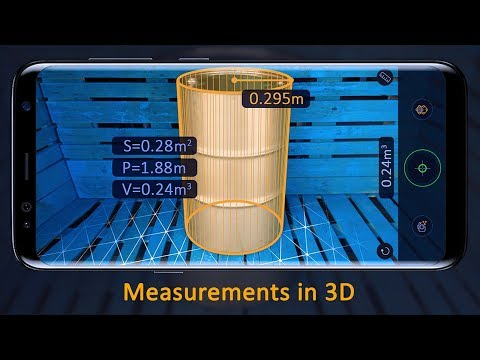
\includegraphics[scale=0.425]{img/measure-app.jpg}
\end{subfigure}%
\caption{Ejemplos de aplicaciones de visión artificial. Google}%
\end{figure}

\section{Autolocalización Visual}
\label{sec:autolocalizacionvisual}

\subsection{Visual SLAM}
\label{subsec:visualslam}

\section{Realidad Aumentada}
\label{sec:realidadaumentada}

\subsection{Tecnologías Software}
\label{subsec:tecnosoftware}

\subsection{Tecnologías Hardware}
\label{subsec:tecnohardware}

\subsection{Aplicaciones}
\label{subsec:raaplicaciones}

\chapter{Objetivos}
\label{sec:objetivos}

\section{Descripción del problema}
\label{subsec:descripcionproblema}

\section{Requisitos}
\label{subsec:requisitos}

\section{Métodología de trabajo}
\label{subsec:metodologiadetrabajo}

\chapter{Estado del arte} %%Buscar el estado del arte que tenemos por ahí
\label{sec:estadodelarte}

\chapter{Infraestructura}
\label{sec:infraestructura}

\section{Elementos hardware}
\label{sec:elementoshardware}

\section{SD-SLAM}
\label{sec:sdslam}

\section{OpenCV}
\label{sec:opencv}

\section{OpenGL}
\label{sec:opengl}

\section{Android}
\label{sec:android}

\subsection{Android Studio}
\label{subsec:androidstudio}

\chapter{SD-SLAM mobile}
\label{sec:desarrollo}

\section{Adaptación de SD-SLAM para Android}
\label{sec:adaptacionsdslam}

\subsection{Incorporación de SD-SLAM a proyecto en Android}
\label{subsec:incorporacionsdslam}

\subsection{Inicialización}
\label{subsec:inicializacion}

\subsection{IMU}
\label{subsec:imu}

\section{AR con OpenGL}
\label{sec:arconopengl}

\chapter{Experimentos}
\label{sec:experimentos}

\section{Guia por flechas}
\label{subsec:guiaporflechas}

\chapter{Conclusiones}
\label{sec:conclusiones}

\cleardoublepage

%\bibliographystyle{abbrv}
%\bibliography{memoria}  

\end{document}
\grid
